\fancyhead[LO]{{\scriptsize 我们最幸福 · 第五章}}%奇數頁眉的左邊
\fancyhead[RO]{\thepage}
\fancyhead[LE]{\thepage}
\fancyhead[RE]{{\scriptsize 我们最幸福 · 第五章}}%偶數頁眉的右邊
\fancyfoot[LE,RO]{}
\fancyfoot[LO,CE]{}
\fancyfoot[CO,RE]{}
\chapter*{第五章 · 维多利亚式的罗曼史}
\addcontentsline{toc}{chapter}{\hspace{11mm}第五章 · 维多利亚式的罗曼史}
\begin{figure}[!htbp]
	\centering
	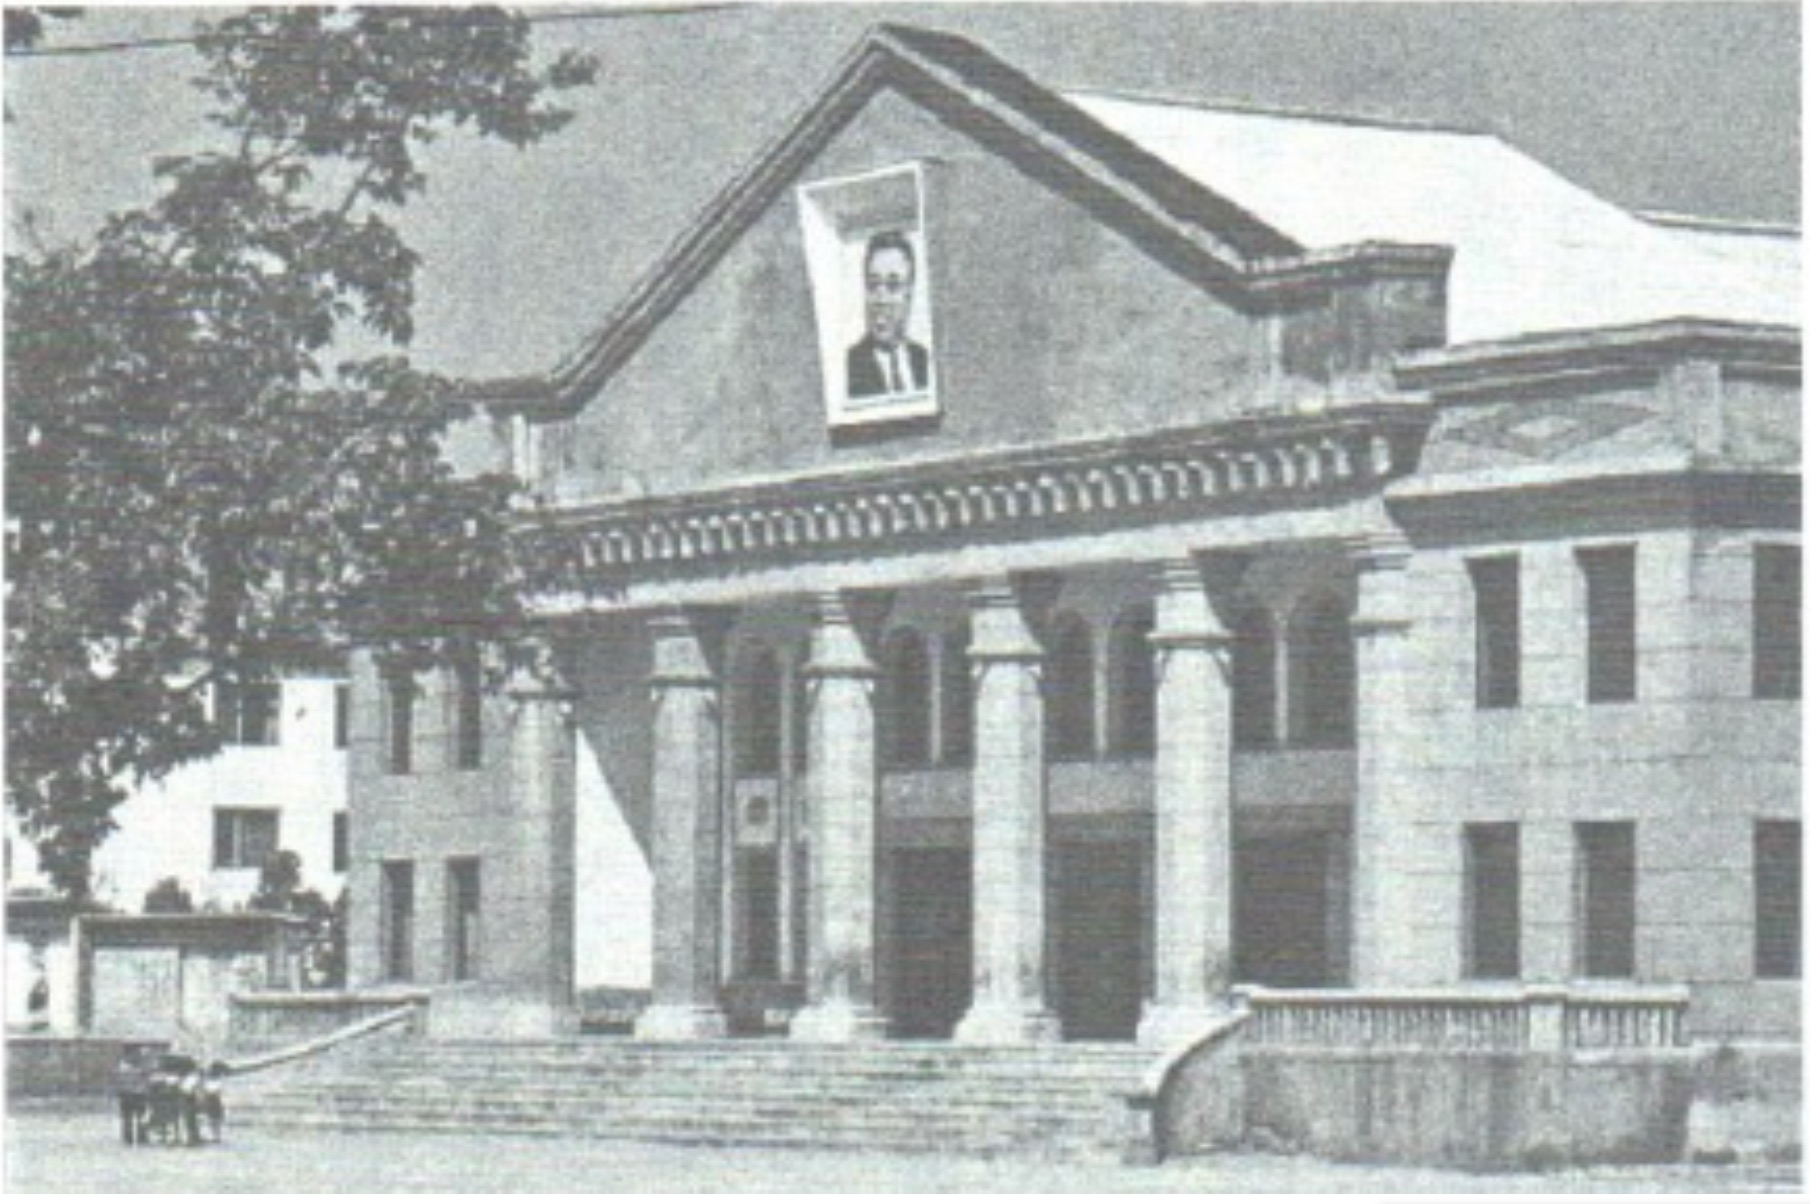
\includegraphics[width=6cm]{./Chapters/Images/05.jpg}
	\caption*{镜城县文化礼堂}
\end{figure}


当第一次注意到城市居民纷纷到乡下去找吃的的时候,美兰还在读高中。她骑车去清津的路上就能看到,他们一个个看上去像乞丐一样,背着个粗麻布袋子,朝路两旁的果园走去。有些甚至走的更远,去到玉米地,去那里要走过她的村子后,再向南朝海边的方向继续走上10公里。城市居民也被发现在美兰父亲工作的高岭土矿附近的山上找柴火。这点颇让美兰感到意外,因为她总认为清津人的生活比镜城人好多了。清津有大学、大剧院、餐馆,这些都是那些劳动党党员及其家属才能去的,像她这样的女孩是不准进去的。\\

镜城其实就是一些村庄围着一个小城区构成的,就像清津一样,只是规模小很多──一条贯穿首尾的大道,一个巨大的石碑,纪念二战中在金日成领导下抗日取得的胜利。还有几个瓷器厂,处理美兰父亲工作的矿生产的高岭土。一个大的电气设备厂,叫六月五日工厂,名字来源于金日成于1948年的那一天,亲临工厂现场指导工作。因此严格来讲,美兰的家并不在乡下,只是相对于城里来说,他们多些土地。靠近海岸的地方,地势平坦,沙质土壤,相对比较肥沃。内陆,地势依次抬升,群山满是茂密的松林。口琴房之间有限的空地,也被人们利用起来,精心的栽种着些红辣椒,白萝卜,大白菜,甚至还有烟草,因为自己卷烟比买的烤烟要便宜,况且几乎每个朝鲜男人都吸烟。家里房子是平顶的人,就在屋顶上放很多瓶瓶罐罐,里面都种着蔬菜。个人的这种小农生产方式因为规模很小,因此也不会触怒共产党当局。至少一开始的时候,在食物短缺还没发展成饥荒的时候,这些小农生产缓解了人们的饥饿。\\

当父亲从矿上拿回家的工资越来越少,并最终消失的时候,美兰母亲就开始了她的冒险。虽然仅仅是个相夫教子的家庭妇女,但是母亲却是个颇有生意头脑的人。她做缝纫,做豆腐,还养了一段时间的猪──后来因没有饲料而无以为继。最成功的还是母亲自己发明的独特配方的仿冰激凌。她先是买了台名叫北极的二手冰箱。因为在北朝鲜你是不可能买到牛奶或奶油的,于是她用做豆腐剩下的汁水加上红豆和糖。再把这看似奇怪的混合物注入冰箱的制冰格里冷冻。朝鲜人很疼爱孩子,如果家有一块余钱他们都会给孩子买好吃的。有时候,美兰的母亲会在一个朋友的卡车后货箱里沿街叫卖她的冰激凌。劳动党的法令禁止私营经济,但是她丝毫不理会。这并不是她有多么叛逆,而是作为一个实用主义者,她从不过多纠缠于所谓的意识形态。卖代冰激凌所赚的钱,能够让她在黑市上买得起所需的玉米,有时候甚至能吃到白米。\\

美兰的秘密男友也没有挨饿。俊相的祖父每年都要乘轮船来北朝鲜看望他们。从90年代早期,轮船不再停靠清津,只停元山──在北朝鲜东海比较靠南的一个港口。俊相一家人就在码头上同祖父见面,每次都是抱在一起,大哭一场,再此期间,俊相的祖父都会偷偷把一个装满现金的信封塞到儿子的口袋里。这必须偷偷的做确保不被政府人员发现,以免事后被他们敲诈。有时候信封里的日元有差不多2000美元之多。在日本的朝鲜人都知道,如果没有这些硬通货,他们在北朝鲜的亲戚就要饿肚子了。\\

俊相家也很幸运,有个私人花园。他父亲非常用心的伺弄着这块地,他把围好的花园分成一个个小块菜地。弓着腰,在花园里劳作着,他像呵护这自己的孩子一样,小心的照顾每一棵幼苗。在一个小本上记下播种的日期,犁土的深度,发芽所需的日子,生长成熟所需的天数。俊相的妈妈有一套买自日本,精致的厨房设备。用锋利的菜刀,她把胡萝卜切成片,白萝卜切成丝,在煮好的饭上面撒些蔬菜丝,再把饭用一片片干的海苔卷起来。他们是邻里之间唯一一家吃Kimbab的,一种在南韩很流行的朝鲜版的日本寿司卷,但是北朝鲜人一般没有见过。有自己种的蔬菜和黑市买的白米,除了劳动党的精英阶层,他们吃的比其它人都有好。\\

家里最值得骄傲的就是俊相自己。多年的苦读,每天晚上学习到凌晨一点,早上天不亮就起床,在父亲无情的鞭策下,自己也希望能完成家庭所寄予的希望,这一切的付出终于得到回报。俊相考入了平壤的一所大学。但不是金日成大学──家庭的成分还不足以达到这个要求──但是这是一所培养科研人员的大学,因此在学生选择上更倾向于有潜质的学生。北朝鲜,在科技方面已经被南韩及日本远远的拉下,已经没有什么本钱去浪费仅有的那些天资聪颖的人才。俊相本来更喜欢文学、哲学,或者影视剧创造也不错,但是父亲却期待他向科学发展,认为那是这个成分不太好的孩子通往平壤的唯一道路。\\

对于一个来自咸镜北道的孩子来说,被平壤相当于北朝鲜的麻省理工的大学录取,那可是件了不起的事情。这也意味着俊相可以免除兵役。现在,他有很好的机会去改善整个家庭的成分──那就是争取加入劳动党。虽然对这个政治体系还是有些疑问──他开始思考,既然共产主义像他们说的那样这么好,为什么东德还要推到柏林墙──但是,确定的是,党员资格和平壤的教育是他通向核心阶层的门票。\\

俊相也为自己的表现引以为荣。他是个谦虚的孩子,一直以来都很小心,不出风头,不显摆自己的聪明和家境,但是那时候,每当他从平壤回家,他总觉得像个衣锦还乡的英雄。同军人一样,大学生被要求穿着校服,即使是在放假离开校园的时候也是。校服是绿色双排扣夹克、裤子、白衬衣还有领带构成。采用绿色是因为金日成曾说过年轻人就像青山一样。春风得意之间,俊相又想约美兰出来。此时距俊相第一次在剧场外遇见美兰已经五年了。让自己不敢相信的是,他仍然忘不了她。在平壤的大学里很多女孩──聪明,漂亮的女孩──但是没人能像美兰那样,让他如此钟情。\\

俊相对美兰已经有些了解。在高中的时候,他就经常讨好美兰的姐姐美淑。美淑比美兰大两岁,是家里的假小子。她参加了女子排球队,经常活动于体育馆附近,而俊相的朋友也在那里训练。俊相还有个在拳击班的朋友,同美兰家住同一排口琴房。俊相以此为借口经常徘徊于她家附近。\\

美兰家设法弄了一台电视,和宋女士家一样,他们也采取开门政策。一天,当俊相去同学家串门的时候,就随着看电视的邻居们一道也晃进了美兰家。当所有人都被电视节目吸引时,俊相却左顾右盼的一会儿看看电视一会儿看看美兰。她已经出落成一个漂亮的姑娘了。他盯着美兰,想仔细看清楚她的眼睛,鼻子,嘴巴还有头发的曲线,想弄明白,为什么这些会让他如此着迷。\\

1991年春天,当第一次从平壤放假回家的时候,俊相决定采取行动。他先是在镜城的中心城区晃荡,希望能和她来个不期而遇,如果那样说不定就有机会和她说上话。在假期的最后一天,他真的等来了机会,在市场上看到她了,然而还没等他走近到可以说话的距离,他猛然看见几步之遥她妈妈就跟在后面。\\

不久,俊相就向美兰的姐姐美淑吐露真情,美淑同意充当他的中间人。在随后的假期里,俊相按约好的时间来到她家。美淑此时正徘徊在门口。“小妹,出来和我朋友说说话。”美淑叫着美兰。\\

美兰把头伸出门外看了看。她尴尬的小声应了一声,又缩回去了。“出来,小妹,不然我就把你拖出来了,”美淑喊道\\

最后,她还是出来见他了。第一次,四目相对,他能感到脑后冒出成串的汗珠,汗湿了刚刚熨烫的制服领子。当他开口说话的时候,他的声音都颤抖着。现在骑虎难下了,他只能硬着头皮往前。他找不到什么话题,只好如实相告。从第一次在剧院外看见她说起。最后,他问她是否能当他的女朋友。\\

“我的学习。我应该用功学习的,但是我不能集中精神,因为我脑子里总是想着你,”他脱口而出。\\

美兰什么都没说。她站在那里,没有像他所期待的那样转过她的目光,但是也没有任何回应。他觉得他的脑袋都要爆炸了。他想方设法的想让她开口。\\

“你没注意到我始终看着你吗?”他问。\\

“没有,真的,我没有注意,”她回答。\\

他没说话,期待着她说下去。\\

“哦,不是说我不喜欢你,”她回答的时候用了一个双重否定的句式,这用朝鲜语表达出来就显得非常模棱两可。他实在闹不清她在说什么,但是隐隐的他觉得,那是一种很小心的积极响应。她后来答应写封信给他,将她的感受写在信里。尽管表面冷若冰霜,其实美兰内心里欣喜万分。她的爱慕者很帅,体贴,老实说,她撞大运了。她认识的男孩里面只有很少几个上了大学,但是没有一个在平壤。虽然她假装吃惊,但是实际上她早就注意到俊相常常出现在自家附近,甚至心理面有时候猜想着他是不是为她而来。穿着闪闪发亮的双排扣制服,他看上去像个海军军官。虽然从没有约会过,但是美兰非常渴望能有个约会。她很纠结如何答应,但是又想保持自己的矜持,不至于显得太渴望答应。结果是信里,字迹工整隽秀,内容却如公文。\\

“如果我不答应使你不快,进而影响你,使你不能集中精力学习,我也不想看到这个局面发生,那么,我就暂时接受你的请求吧,”她几周之后这样写道。\\

尽管是以一种19世纪的鸿雁传书的方式,两个人总算开始交往了。他们两人之间唯一的联系方式就是写信,此时是1991年,南韩已经成为世界上最大的行动电话出口国家,同时大部分北朝鲜人却连电话都从未使用过。要打电话,你要去邮局。然而,就算是写信,也非易事。因为信纸很难得。通常人们都是在报纸的空白处写东西。商店卖的纸张都是用玉米秆做的,稍微用点力就会写破。美兰之后向妈妈讨些钱买几张进口的纸。进口的纸张就怎么划都没问题;因此纸也要省着用。平壤与清津仅仅相距400公里,但是信件要花上1个月才能收到。\\

当他们开始的时候,是美兰高中的最后一年。相对于男友的大学生背景,美兰倍感压力。在平壤,俊相买得到不错的信纸。他还有支圆珠笔,他的信通常都是好几页,洋洋洒洒的,文笔非常好。他们之间的通信内容也慢慢从礼节性的客套,慢慢过度到情意绵绵的浪漫。俊相从来没看过好莱坞式的浪漫电影,但是他现在被爱情冲昏头脑,满脑子都是那些经典爱情场景。他曾经在给美兰的信中描绘,在天空美丽的彩霞下,他和美兰跑向一起。他像她讲述这自己在平壤看的小说。他写情诗给她。在纸上,多年以来想对她说的话终于得以一吐衷肠。\\

俊相把信寄给美淑,此时美淑已经工作了,因此通过把信寄到美淑的办公室可以避免她父母的察觉。美淑是家里唯一知道这件事的人。俊相也是守口如瓶。其实,他们之间从没有刻意的提到要保守秘密,因为他们都明白在北朝鲜性和家庭成分都是讳莫如深的话题──实际上抱怨自己的成分songban,就是对当局不满。美兰出生不好,这对双方是不言而喻的。他们两个都心知肚明,如果他们真的结婚了,这对俊相的前途不利,而他加入劳动党的梦想也要化为泡影。当然,如果俊相的父亲发现了,他也会棒打鸳鸯的。北朝鲜社会讲究人们遵从长辈。俊相明白他父母期望他找个同是朝鲜日本归侨出身的女孩。因此无论如何,俊相的父亲都不会准许他去约会的。\\

“先把书读完。不要把时间浪费在追女孩上面,”他教训道。\\

这里先谈谈性在北朝鲜这个话题:这个国家没有什么约会的传统。很多婚姻仍然是包办婚姻,或者是由家庭包办或者是由党书记或者领导安排的。情侣们也不习惯于大庭广众之下卿卿我我──甚至连公开牵手都被视为伤风败俗。脱北者都坚称在北朝鲜没有婚前性行为,也没有未婚女学生怀孕的事情发生。“那将是无法想象的灾难。我几乎不敢想象这样的事情真的会发生,”一个已经矜持不再的逃北妇女是这样告诉我的,当我遇见她的时候,她在首尔以出卖肉体为生。显然,在北朝鲜也没有南韩或日本那种情人旅馆。没有旅行许可,你甚至都普通旅馆都无法登记入住,就更不会有旅馆允许未婚男女同处一室了。清津来的人告诉我,未婚情侣如果情不自禁,那只能去野外或者晚上去公园,但是从没有人听说有人承认这么做过。\\

女子举止得体,洁身自好是传统朝鲜文化所推崇的。当你置身于首尔街头,满眼都是女学生的花格子超短裙,你很难想象仅仅一个世纪以前,这里的妇女是从头包到脚,和塔利班统治下的妇女如出一辙。19世纪英国旅行家伊萨贝拉伯德大主教曾经描写1897年她在平壤以北一个小村庄里,看到妇女们都穿着一种类似长袍的奇怪的衣服,她是这样描述的“那怪异的帽子看上去正如花园里的岗亭,但是没有底。这个看上去奇奇怪怪的东西,有220公分长,165公分宽,深90公分,把人像木乃伊一样从头裹到脚。中上阶层人家的女人不允许抛头露面,除非在一些特定的时刻,而那时候街上的男人都要回避。大主教曾经常游历于伊斯兰世界,即便如此,她仍宣称朝鲜妇女受到“最严酷的束缚,世界范围之内,实属登峰造极了。”\\

历史早已不复存在,然而传统观念却得以留存。金日成掌权之后,他将朝鲜传统与共产主义天然对性的压抑相结合。他不仅关闭妓院,而且更进一步,连那些服务于富人的艺伎也一并取缔。创造淫秽作品将被处决。除了他自己和儿子──年轻时曾是花花公子的金正日,可以为所欲为,其它人即便是党干部,如果被发现有奸情,也将被罢黜。\\

金日成对早婚也不提倡,并于1971年发出“特别指示”规定男性应不早于30,女性不早于28岁结婚。北朝鲜报纸曾这样报导,“祖国希望,也相信年轻人将遵循传统美德,在对国家做出足够贡献后再结婚。”事实上,这根本不是什么朝鲜传统──在过去,朝鲜人一般在十四就就要谈婚论嫁了。这项规定原本是用于提升军人士气,有了这个规定,他们不用担心自己的女友等不及自己服完兵役了。然而,晚婚也降低了婴儿出生率。虽然这道禁令于90年代取消,然而北朝鲜人仍然对成双成对的年轻人嗤之以鼻,虽然他们可能根本就是普通朋友。\\

宣传运动也倡导妇女选择“符合社会主义生活方式和体现时代气息的发型。”对于中年妇女,这就意味着是烫卷的短发。未婚女性则可以留长发,但是必须扎在脑后或者编成辫子。北朝鲜妇女也不允许穿高于膝盖的裙子,或者无袖衫。有趣的是,南韩在70年代,朴正熙军事独裁时代也曾有过类似的规定。而现在南韩却已经发生了翻天覆地的变化,从这点也侧面反映了北朝鲜整个社会还停滞在什么年代,同文同种的两种不同的文化对待穿着和性的态度已经是天壤之别了。几年前,当我前往当时非常热门的北朝鲜境内对南韩游客开放的旅游区时,我注意到北朝鲜宾馆的门童看到南韩游客里年轻姑娘穿着低腰牛仔裤和露脐装的时候,他们几乎要昏厥的表情。很多我访问过的脱北者告诉我,当他们来到南韩的时候,最让他们吃惊的就是年轻人在大庭广众之下接吻。\\

因此,虽然电力短缺带来诸多不便,俊相和美兰却也因此有机会开始发展。北朝鲜夜间的黑暗是那种生活在电气化世界的人们从未经历的,那种黑暗无法相信。没有街灯,没有汽车头灯,没有任何光线从窗户,门下透出来,那种黑暗就像是被一层厚厚的东西包裹着,没有一丝光线。在大街上,只有当你看到一个人吸着的烟头那点亮点,你才能知道有个人沿着街道走过来了。\\

吃完晚餐,俊相就会找个借口出来。虽然他已经是20岁的大学生,个子也比父亲高一个头,可是他仍然对父亲心存畏惧。\\

“我出去找个朋友,”俊相边说边出了门,随便的提了这个或者那个高中好友的名字。他答应晚上9点之前回家,但是他明白不到半夜是回不来的。然后他又会找些借口来搪塞他父亲。\\

去美兰家,大概步行要半个小时。他走的很快,虽然他知道到了之后可能是长时间的等待,因为美兰没有帮她母亲收拾完晚餐后的家务之前是出不来的。而且他现在也找不到什么借口在她家周围逛荡,他那个拳击班的同学,也就是她的邻居,早就搬家了。所以他只能待在黑暗里,安静的等着,静的他觉得甚至能听见自己的心跳。\\

那时候,就那么几个约会能去的地方早就关门了。镜城文化礼堂因为没电,电影放映机无法运转。早些年还开放的,仅有的几个餐馆现在也是关门大吉了。清津城区沿着海边在码头的旁边,就是清津青年公园,里面有个湖,可以划船,还有个破烂不堪的游乐场,然而旅行证查的很严,从郊区去城里也要旅行许可。他们也不敢去火车站后面的镜城公园,害怕在哪里会遇到熟人。\\

所以,长途步行也就成了最好的选择。其实,路也只有一条,从城里通往山区。他们也是尽可能轻快的走,不要表现的好像是逃跑一样。当他们走过微笑的金日成标语牌之前是不说话的,标语牌写着“如果党决定了,我们就坚决执行。”以及“让我们用生命护卫金正日。”还有一个彩色标语牌上是一个拿着刺刀的士兵竖在街道的一边,街道在这里从一个点缀这蓝花的天桥下穿过。当路两旁的标语牌开始变少的时候,那就是出城了。在黑暗中,他们也可以放松警惕了。黑暗里,他们的瞳孔会放大,这样用不着凝视就可以看到夜景。道路两旁,行道树高大茂盛的,枝叶繁盛,在头顶上形成一个天然的蔽阴华盖。在晴朗的夜空中,星星点点的星光从树枝间穿透下来。再走几分钟,道路开始上坡了,整个村庄也就展现在路旁,而另一侧这是陡峭的山坡。茂密的松树林覆盖着山腰,树林里左一丛,右一簇的在岩缝里开满紫色的野花。\\

然后,道路跨过一条两边是沙堤的小溪后突然向左边急拐,之后就通向Onpho温泉度假村,这个地方的温泉是朝鲜唯一的碱性温泉,温泉水温常年保持在55度,据传此温泉能包治百病,从消化不良到不孕不育无所不能。再往前,路就被一个检查站封锁,那里就是金日成的别墅──据说是金日成在全国所建的,供他随时享用的三十个别墅中的一个。那里,戒备森严,普通人不允许游荡于附近。虽然不对外开放,但是从路上却可以看到里面有个党干部专用的温泉浴场。而对公众开放的温泉浴场也因经济困难,勉力支撑,浴场里那些石砌的,混凝土的建筑也都年久失修。度假村最早于1946年开放,有一幅画描绘当时落成时的场景,在画中金日成被一群医生拥簇着,现在度假村看上去,好像从那时起就从未得以任何维护。度假村前面一个巨大空地,杂草丛生,晚上看上去十分空旷。这对年轻人对眼前景象没什么兴趣,两人能在一起才是最重要的,即便在夜晚走了几公里,脚板酸痛也是值得的。\\

边走,边说,这就是他们约会,仅此而已。谈话是那么生动有趣,时间在不知不觉中慢慢流逝。当面对面的时,俊相却没有了信里浪漫的勇气。他很礼貌,文雅,甚至不敢牵美兰的手,俊相直到两人约会3年后,才第一次牵手美兰。他给她讲故事,讲他们朋友,宿舍。他告诉她当学生们在操场上点名时,学生们是怎么样被编排队列,队列行进时手脚如何步调一致。他还向她讲述着在平壤的见闻,美兰只去过平壤一次,那还是小学里,去参观纪念碑。平壤可是代表着现代的缩影──如宣传所称,这个城市的建筑及其在技术水平方面上所取得的成就是世界上最伟大的。俊相告诉她,双子塔的高丽饭店顶上有个旋转餐厅。他从来没进去过那里,只是曾久久凝视着地平在线它的轮廓,在天际在线它和高达一百零五层的金字塔形的,号称亚洲最大建筑的柳京饭店遥相呼应。俊相还向她描述平壤的地铁,那可是在深达90米的地下,地铁站里装饰着大吊灯,还有镀金的马赛克拼成的金日成像。\\

回平壤后,俊相去了外汇商店,用他的日元给美兰买了一个蝴蝶形镶着一排排水钻的发夹。对美兰来说,这个发夹真让她眼花缭乱,又充满异国情调──她还从来没有拥有过如此精美的东西。因为不想引起母亲的询问,她从没有佩戴过它。只是小心翼翼的把它藏在自己的内衣里面。\\

俊相在平壤的经历,使得美兰得以一窥遥远的特权世界是怎个样子。同时,她还要装作很平静的听,不要表现出任何的嫉妒。她高中即将毕业了,她有预感这自己做学生的日子到头了。她曾经目睹自己的姐姐们一个个曾经满怀信心,仅仅因为自己父亲的历史,而最终都以失望而告终。甚至连参加大学的入学考试都需要得到当地教育委员会的许可。她的三个姐姐只有大姐进入了学院,而且不是她心仪的艺术表演专业,白白浪费了一副天生的好嗓子。大姐进入的是体育专业,后来也因结婚也半途而废。\\

美兰早就清楚自己的未来会是怎样。她甚至已经能看到她前面的路,平淡无奇──进入工厂,结婚(很可能就同厂子里的工人),生孩子,衰老,死去。然而,当俊相闲聊着他的大学同学时,她内心却越来越痛苦。俊相感觉到了她内心的细微变化,慢慢开导她,使她终于向他敞开心扉。\\

“我觉得我活着毫无意义,”她脱口而出。\\

他略有所思的听着。几周后,他回到平壤就给她写了封信。\\

“任何事情都不是一成不变的,”俊相在信中写道。“如果你想改变命运,那么你就必须首先要相信自己,通过努力你能梦想成真。”\\

后来,美兰一直以俊相的话激励着自己去改变命运。她曾经是个好学生,就因心灰意冷,成绩一落千丈。如果前途渺茫,自暴自弃又有什么区别?但是俊相的一席话,惊醒梦中人。她拾起书本,央求母亲让她从繁重的家务中解脱出来,以便她能有时间学习功课。她请求老师能够允许她参加大学的入学考试。如果真的事与愿违,进不了大学,她也没什么遗憾得了,至少她努力了。\\

出乎意料的是,她被师范学院录取了。金正淑师范学院──以金正日母亲的名字命名的学院,是清津最好的师范学院。为什么她这么幸运而姐姐们都失败了呢?美兰自己也觉得奇怪,因为她自认为虽然是属于好学生,但是在班上都算不上顶尖。她原以为那些家庭出生好的,成绩也不差过她的女孩应该早就把招生名额占满了。\\

在1991年的秋天,她搬出了父母的家,搬进了大学集体宿舍。学校在市里的浦项区,就在博物馆的对面,前面有金日成雕像的公园的后面。\\

第一次到宿舍,给美兰留下深刻影响。宿舍非常现代化了,每四个女孩住一间宿舍,每个人都配有一张床,而不是在朝鲜传统的那种暖炕上的席地而睡,其实以传统的方式可以用最少的燃料就保证整晚都很暖和。到了冬天,当清津的天气天寒地冻的时候,美兰总算弄明白了为什么她在新生里会有一席之地。宿舍没有暖气系统。美兰每晚睡觉都穿着大衣,厚袜子,手套,还要用毛巾罩住头。每天早上,当起床的时候,呼出的水汽在毛巾上冻成了霜,使得毛巾都变得很脆。在水房,女孩们在那里洗月经带\footnote{那时没人有卫生巾,条件好些的女孩用纱布绷带,而穷的就只能将就着用廉价的化纤布。},天气冷得出奇,洗好的挂在那里晾干的月经带几分钟就冻得硬梆梆的了。美兰最恨的就是早上。同俊相的学校一样,美兰的学校也实行军事化管理,每天早上六点起床,但是不像自豪的士兵出操,她们都是哆哆嗦嗦的挪进水房,朝脸上泼着刺骨的冰水。在冻得硬邦邦的月经带下,女孩子们钻来钻去。\\

相对于住宿条件,食堂的饭菜就更差的了。当时,北朝鲜正在开展一项运动“让我们每天只吃两顿”,但是学校把这项运动开展的更彻底,每天只提供一顿餐饮──一份汤,就是一点盐,几片萝卜干加点水而已。有时候,食堂也会加一勺煮了几个小时变得又大又泡的米饭或者玉米。学院里的女生开始一个接一个的病倒。美兰的一个室友因为极端营养不良,脸上除了皮就是骨头了。她最后退学了,很多人也接着一个个退学。\\

值得一提的是,美兰在勤劳母亲的荫庇下,得以度过此次经济危机。她央求母亲从家里拿些吃的给她,然而一年后,家里也拿不出什么了。由于不想就此而放弃她千辛万苦得来的受教育的机会,她得到学校的允许,住在校外。这样她一个星期平常的时候住在一个亲戚的家中,周末的时候就回家。通常这样是不允许的,但是学院的行政管理部门现在也是能少一张嘴就少一张了。\\

俊相在平壤的日子相对容易些。政府在给养上给这些精英的学生以最高优先权,这些学生可是明日的科学家,政府也将未来解决北朝鲜贫困的希望寄托在他们身上。俊相仍然每天三顿集合后集体进餐。他们的宿舍晚上仍然有暖气,有电,这样他们在天黑之后仍可以学习。\\

俊相和美兰只能在俊相一年两次的寒暑假里才能见面,除此之外,仅有春假有机会见面,春假里学生们被组织去地里除草,以备播种。在过去,平壤的学生就在首都郊外的田里完成任务,但是随着食物短缺,学校决定让学生们回家,在家乡参加劳动,这样就可以在家解决吃的问题。俊相向来很担心这项田里的志愿劳动,现在他却盼着从学校放假回家的日子。这种渴望也是一种发泄,多年来他只是读书学习。“我真的想放弃一切,回家见她。我第一次意识到,在我生命里什么才是人类的感情,”他后来是这么描述那段时期的。\\

在1993年秋天,俊相的姐姐结婚。虽然他父母已经叮嘱过他,不要因此影响他的学习,但是俊相想这可是个绝好的借口给美兰一个惊喜。于是他还是请了3天假回了家。此时,平壤往北开的火车已经很少了,因为火车都是靠电驱动。即使想方设法弄到了票,除非是党高级干部,一般都是无坐的。火车站里也挤满了等车的旅客。他们都在黑暗里,或是四处闲逛,或是蹲着吸烟,等着火车到站。一旦有车来了,他们就不顾一切的冲过去,从破了的窗口爬进车厢,或者有的就挂在车厢之间。\\

由于买不到票,俊相只好等在车站,看看有没有过路车。一天之后,他才发现有一列北上的货车。用了几支烟送给一个机修工,才得知这趟车会经过清津。因此他爬到运煤的车皮上,用一条毛巾裹着脸以保护眼睛。这是他这辈子第一次这样扒货车回家,但是不是最后一次。\\

清津的前一站是镜城──离美兰的村子不远。俊相在那里跳下了车,径直跑去了她家。与往常见面时间不同的是,这次是上午时分艳阳高照,但是他却等不及了。他觉得如果要等到天黑,那他会发疯的。那天正好是周日,他猜想美兰应该在家,所以自从秘密幽会以来,第一次他站在了美兰家的大门口。\\

门开了,美兰的妈妈向外张望。\\

俊相的脸就像他的衣服一样,满是煤灰。美兰的妈妈认识俊相,因为他同其它一些邻居的孩子来过几次,但是现在她却认不出他来了。还好,美兰当时不在家。\\

“有个奇怪的人来找你,”美兰的妈妈后来告诉她。“你朋友都是些什么奇怪的人啊。”\\

他们险些就被母亲撞破。俊相那边,他父亲对儿子中断学习回来参加姐姐的婚礼很不高兴,并质问他的目的。俊相后来在一个晚上进到美兰家里,那晚美兰的父亲去矿上上夜班,而母亲也出去了。但是,后来美兰的父亲却突然回来了,俊相只好藏起来,直到外面安全了才出来。\\

后来,俊相和美兰回忆起这个惊险的意外,还大笑不止。事实上,他们都很享那个时候瞒着父母的时光。保密不仅是必须的,有时候也很有趣。在一个没有隐私的社会里,这使得他们整天提心吊胆,偷偷摸摸的,然而也正是这样使他们得以分享相互之间的心灵感应。同时,这也是一种相对安全的,对束缚的抗争。\\

他们越聊,笑的也越多。后来,当年长了些,也在舒适安全的环境下,再回首那么日子,他们都认为那是一生中最快乐的时光。在被爱情冲昏头脑的时候,他们对周围发生什么也就不太很注意。\\
